%% For distribution of the original source see the terms
%% for copying and modification in the file samples.dtx.
%% 
%% This generated file may be distributed as long as the
%% original source files, as listed above, are part of the
%% same distribution. (The sources need not necessarily be
%% in the same archive or directory.)
%%
%%
%% Commands for TeXCount
%TC:macro \cite [option:text,text]
%TC:macro \citep [option:text,text]
%TC:macro \citet [option:text,text]
%TC:envir table 0 1
%TC:envir table* 0 1
%TC:envir tabular [ignore] word
%TC:envir displaymath 0 word
%TC:envir math 0 word
%TC:envir comment 0 0
%%
%%
%% For submission and review of your manuscript please change the
%% command to \documentclass[manuscript, screen, review]{acmart}.
%%
%% When submitting camera ready or to TAPS, please change the command
%% to \documentclass[sigconf]{acmart} or whichever template is required
%% for your publication.
%%
%%
\documentclass[acmsmall, review, screen]{acmart}

%%
%% \BibTeX command to typeset BibTeX logo in the docs
\AtBeginDocument{%
  \providecommand\BibTeX{{%
    Bib\TeX}}}

%% Rights management information.  This information is sent to you
%% when you complete the rights form.  These commands have SAMPLE
%% values in them; it is your responsibility as an author to replace
%% the commands and values with those provided to you when you
%% complete the rights form.
\setcopyright{acmcopyright}
\copyrightyear{2022}
\acmYear{2022}
\acmDOI{XXXXXXX.XXXXXXX}

%% These commands are for a PROCEEDINGS abstract or paper.
\acmConference[Conference acronym 'XX]{Make sure to enter the correct
  conference title from your rights confirmation emai}{June 03--05,
  2018}{Woodstock, NY}
%%
%%  Uncomment \acmBooktitle if the title of the proceedings is different
%%  from ``Proceedings of ...''!
%%
%%\acmBooktitle{Woodstock '18: ACM Symposium on Neural Gaze Detection,
%%  June 03--05, 2018, Woodstock, NY}
\acmPrice{15.00}
\acmISBN{978-1-4503-XXXX-X/18/06}


%%
%% Submission ID.
%% Use this when submitting an article to a sponsored event. You'll
%% receive a unique submission ID from the organizers
%% of the event, and this ID should be used as the parameter to this command.
%%\acmSubmissionID{123-A56-BU3}

%%
%% For managing citations, it is recommended to use bibliography
%% files in BibTeX format.
%%
%% You can then either use BibTeX with the ACM-Reference-Format style,
%% or BibLaTeX with the acmnumeric or acmauthoryear sytles, that include
%% support for advanced citation of software artefact from the
%% biblatex-software package, also separately available on CTAN.
%%
%% Look at the sample-*-biblatex.tex files for templates showcasing
%% the biblatex styles.
%%

%%
%% The majority of ACM publications use numbered citations and
%% references.  The command \citestyle{authoryear} switches to the
%% "author year" style.
%%
%% If you are preparing content for an event
%% sponsored by ACM SIGGRAPH, you must use the "author year" style of
%% citations and references.
%% Uncommenting
%% the next command will enable that style.
%%\citestyle{acmauthoryear}

%% Packages
\usepackage{xcolor}
\usepackage{color}
\usepackage{listings}

%% Custom Definitions
\graphicspath{{graph/}}
\definecolor{ForestGreen}{HTML}{009B55}

\lstset{inputpath=code_examples/src/Examples}
\lstset{
  frame=none,
  xleftmargin=2pt,
  stepnumber=1,
  numbers=left,
  numbersep=5pt,
  numberstyle=\ttfamily\tiny\color[gray]{0.3},
  belowcaptionskip=\bigskipamount,
  escapeinside={*'}{'*},
  language=haskell,
  tabsize=2,
  emphstyle={\bf},
  commentstyle=\color{ForestGreen},
  stringstyle=\mdseries\rmfamily,
  showspaces=false,
  keywordstyle=\bfseries\rmfamily,
  columns=flexible,
  basicstyle=\small\sffamily,
  showstringspaces=false,
  morecomment=[l]\%,
}

%% CUSTOM PACKAGES - NON-ACCEPTED
\usepackage{todonotes}

%%
%% end of the preamble, start of the body of the document source.
\begin{document}

%%
%% The "title" command has an optional parameter,
%% allowing the author to define a "short title" to be used in page headers.
\title{LayeredTypes}

%\title[LayeredTypes]{Layered Types -- An approach to arbitrarily combine LiquidTypes in a structured Manner}

%%
%% The "author" command and its associated commands are used to define
%% the authors and their affiliations.
%% Of note is the shared affiliation of the first two authors, and the
%% "authornote" and "authornotemark" commands
%% used to denote shared contribution to the research.
\author{Lukas Abelt}
\email{l.abelt@luabelt.de}
\orcid{1234-5678-9012}
\affiliation{%
  \institution{Saarland University}
  \streetaddress{XXX}
  \city{Saarbrücken}
  \state{Saarland}
  \country{Germany}
  \postcode{66113}
}

%%
%% By default, the full list of authors will be used in the page
%% headers. Often, this list is too long, and will overlap
%% other information printed in the page headers. This command allows
%% the author to define a more concise list
%% of authors' names for this purpose.

%%
%% The abstract is a short summary of the work to be presented in the
%% article.
\begin{abstract}
	\todo[inline]{Write useful abstract}
\end{abstract}

%%
%% The code below is generated by the tool at http://dl.acm.org/ccs.cfm.
%% Please copy and paste the code instead of the example below.
%% TODO
\begin{CCSXML}
<ccs2012>
 <concept>
  <concept_id>10010520.10010553.10010562</concept_id>
  <concept_desc>Computer systems organization~Embedded systems</concept_desc>
  <concept_significance>500</concept_significance>
 </concept>
 <concept>
  <concept_id>10010520.10010575.10010755</concept_id>
  <concept_desc>Computer systems organization~Redundancy</concept_desc>
  <concept_significance>300</concept_significance>
 </concept>
 <concept>
  <concept_id>10010520.10010553.10010554</concept_id>
  <concept_desc>Computer systems organization~Robotics</concept_desc>
  <concept_significance>100</concept_significance>
 </concept>
 <concept>
  <concept_id>10003033.10003083.10003095</concept_id>
  <concept_desc>Networks~Network reliability</concept_desc>
  <concept_significance>100</concept_significance>
 </concept>
</ccs2012>
\end{CCSXML}
%TODO
%\ccsdesc[500]{Computer systems organization~Embedded systems}
%\ccsdesc[300]{Computer systems organization~Redundancy}
%\ccsdesc{Computer systems organization~Robotics}
%\ccsdesc[100]{Networks~Network reliability}

%%
%% Keywords. The author(s) should pick words that accurately describe
%% the work being presented. Separate the keywords with commas.
%TODO: Keywords
\keywords{}
%% A "teaser" image appears between the author and affiliation
%% information and the body of the document, and typically spans the
%% page.
\begin{teaserfigure}
  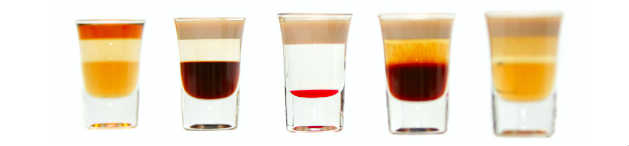
\includegraphics[width=\textwidth]{layered-shots.jpg}
  \label{fig:teaser}
\end{teaserfigure}

\received{20 February 2007}
\received[revised]{12 March 2009}
\received[accepted]{5 June 2009}

%%
%% This command processes the author and affiliation and title
%% information and builds the first part of the formatted document.
\maketitle

\section{Introduction}
\subsection{Context}
Using Refinement Types allows us to define contracts for function types that define pre-conditions on the function arguments and post-conditions on it's return values. These contracts can then be checked statically at compile time. One implementation of this is LiquidHaskell. When combining function calls, it can be verified that the post-condition of the inner function will also fulfill all pre-conditions of the outher function. Listing \ref{lst:liquidhaskell} shows an example of this.

\lstinputlisting[language=Haskell,caption={Contracts in LiquidHaskell}, label={lst:liquidhaskell}]{BasicLT.hs}

Using these contracts, the programmer can clearly define the expectations and assurances that are made to the functions they write. Ensuring their fulfillment before code execution can have a great impact on a programs correctness and stability.

\subsection{Motivation}
One challenge current implementations of LiquidTypes face is that is is not always possible to trivially combine different constraints. Assume that in LiquidHaskell we have two refinement types for non-empty and ordered lists respectively. Freely combining these two types is not possible, so we rather have to create a new, separate, refinement type for this as shown in Listing \ref{lst:combined_refs}. 

\lstinputlisting[language=Haskell,caption={Combining Refinement Types},label={lst:combined_refs}]{CombinedLT.hs}

As we have to combine the two constraints into one refinement type they are also always checked together. While this seems like a non-issue for simple functions as the ones presented so far, this may hinder the programmers ability to identify which pre-conditions are not ensured when writing functions that interface with already existing code. Assume that some developer writes a function whose result he wants to pass to the \texttt{maxVal} function defined in Listing \ref{lst:combined_refs}.

\subsection{Problem Definition}
\subsection{Impact}
\subsection{Approach}
\subsection{Contributions}
\section{Related Work}
\section{Background}
\section{Implementation}
\section{Evaluation}
\section{Conclusion}
\section{Acknowledgments}

\end{document}
\endinput
%%
%% End of file `sample-acmsmall-conf.tex'.
